% !TEX root = ../main.tex

% Project report section

\section{Project report}
\subsection{Background}
Bayesian Optimization (BayesOpt) is a widely-used framework for finding global optima of expensive, black-box functions \cite{Jones1998, Frazier2018, Garnett2023}. While multiple software implementations exist, the BoTorch Python library \cite{Balandat2019} and the DiceOptim R package \cite{Roustant2012} are two popular choices. Here, we report a simulation study comparing these software implementations across different objective functions, using different acquisition functions. We compare both optimization performance (how close to the global optimum each method reaches) and computational efficiency (how long each method takes to run). Our results suggest that BoTorch represents a safe default implementation and that the Knowledge Gradient acquisition function often provides the most favourable results.

\subsection{Methods}
The performance and efficiency of BayesOpt implementations were assessed using the Gap measure as defined in (\ref{gap}) and the time per iteration in seconds, respectively. Here one ``iteration'' comprises optimizing the acquisition function, evaluating the objective function at the acquisition optimizer point, and updating the Gaussian Process model given the new observation. The implementations compared were BoTorch (v. 0.10.0) and DiceOptim (v. 2.1.1) \cite{Roustant2012, Balandat2019}. Standardized versions of the Hartman 6 (H6), Rosenbrock 4 (Ros4), and Goldstein–Price (GP) test functions were implemented in Python following their validated R implementations in the DiceOptim and DiceKriging (v. 1.6.0) R packages\footnote{DiceKriging and DiceOptim were published together as complimentary R packages \cite{Roustant2012}.}. Specifically, the original functions were modified as necessary so that the input space ranged from 0 to 1 for all input dimensions. No validated implementation of the Shubert test function was available and, therefore, this test function was not used. All simulations employed noise-free observations of each test function.

Both BoTorch and DiceOptim implementations employed a Matérn kernel ($\nu=5/2$). Based 
on availability, Expected Improvement (EI), Knowledge Gradient (KG), and (log) Probability of Improvement (LPI, defined in \href{https://botorch.org/api/acquisition.html\#botorch.acquisition.analytic.LogProbabilityOfImprovement}{BoTorch}) were used as acquisition functions for BoTorch, and only EI and KG were used for DiceOptim. Predictive Entropy Search was unavailable in both BoTorch and DiceOptim. Acquisition functions were optimized using the L-BFGS-B algorithm. The remaining parameters employed default values from each implementation.

A total of 100 simulation repetitions were run for each simulation scenario. Each simulation run consisted of an independent run of BayesOpt with a given set of implementation (BoTorch vs. DiceOptim), acquisition function (EI, KG, or PI), and test function (H6, Ros4, and GP). Within each run, an initial GP model was fit to $n_0=10$ observations of the corresponding test function, evaluated at points sampled uniformly at random from the input space; BayesOpt was then carried out for $n=30$ iterations. The relatively high $n_0$ was necessary to avoid numerical problems with DiceOptim, which employs Maximum Likelihood Estimation by default. The relatively low $n$ was chosen due to time limitations.

Finally, a ``negative control case'' was also assessed: instead of selecting the next evaluation point based on the acquisition function, we sample a point from the input space uniformly at random. This is intended as a minimal baseline to be outperformed by the actual BayesOpt methods.

All analyses are fully reproducible with as few as two commands with code from the GitHub repository \href{https://github.com/giulianonetto/qp-giulianonetto-bayesopt}{https://github.com/giulianonetto/qp-giulianonetto-bayesopt}, based on a fixed Docker image \cite{merkel2014} with Python (3.10) and R (v. 4.3.2).
\subsection{Results}
Gap and running time results were recorded across 100 simulation runs. The estimated mean Gap values per objective function evaluation (iteration) alongside corresponding 95\% confidence intervals (CI) are shown in Figure (\ref{fig:gap}). At a given iteration number, a higher mean Gap value means the optimization procedure reached closer to the global optimum, on average. Optimization performance varied substantially depending on test and acquisition functions as well as on the choice of implementation.

As expected, the mean gap increased slowly with iteration when the next evaluation point of the input space was chosen randomly -- the ``Random'' curves in Figure (\ref{fig:gap}). Yet, random input choice showed substantially different mean gap values at iteration 1 across different test functions, reflecting varying optimization difficulty. Its performance was particularly high for the Rosenbrock 4 test function, leaving little room for improvement through BayesOpt.

Still, the BoTorch implementation outperformed random input choice after 5 or 10 iterations across all test and acquisition functions. The benefit was most notable for the Hartman 6 function, in which case Expected Improvement and (log) Probability of Improvement performed better at initial iterations but were clearly surpassed by Knowledge Gradient after 15 iterations. Though to a lesser extent, a similar dependency of the best acquisition function on the iteration number was also observed for the Goldstein-Price test function. After all 30 iterations, the mean Gap for Knowledge Gradient was reasonably high for all three test functions, while Expected Improvement and (log) Probability of Improvement reached comparable performance for the Rosenbrock 4 and Goldstein-Price functions only. No major performance differences were observed between Expected Improvement and (log) Probability of Improvement.

Results were surprisingly different for the DiceOptim implementation. In this case, BayesOpt provided a clear benefit over random input choice for the Goldstein-Price test function only, particularly when employing Knowledge Gradient. For both Hartman 6 and Rosenbrock 4 functions, DiceOptim showed mean Gap values comparable to randomly choosing evaluation points, regardless of the acquisition function.

\begin{figure}[H]
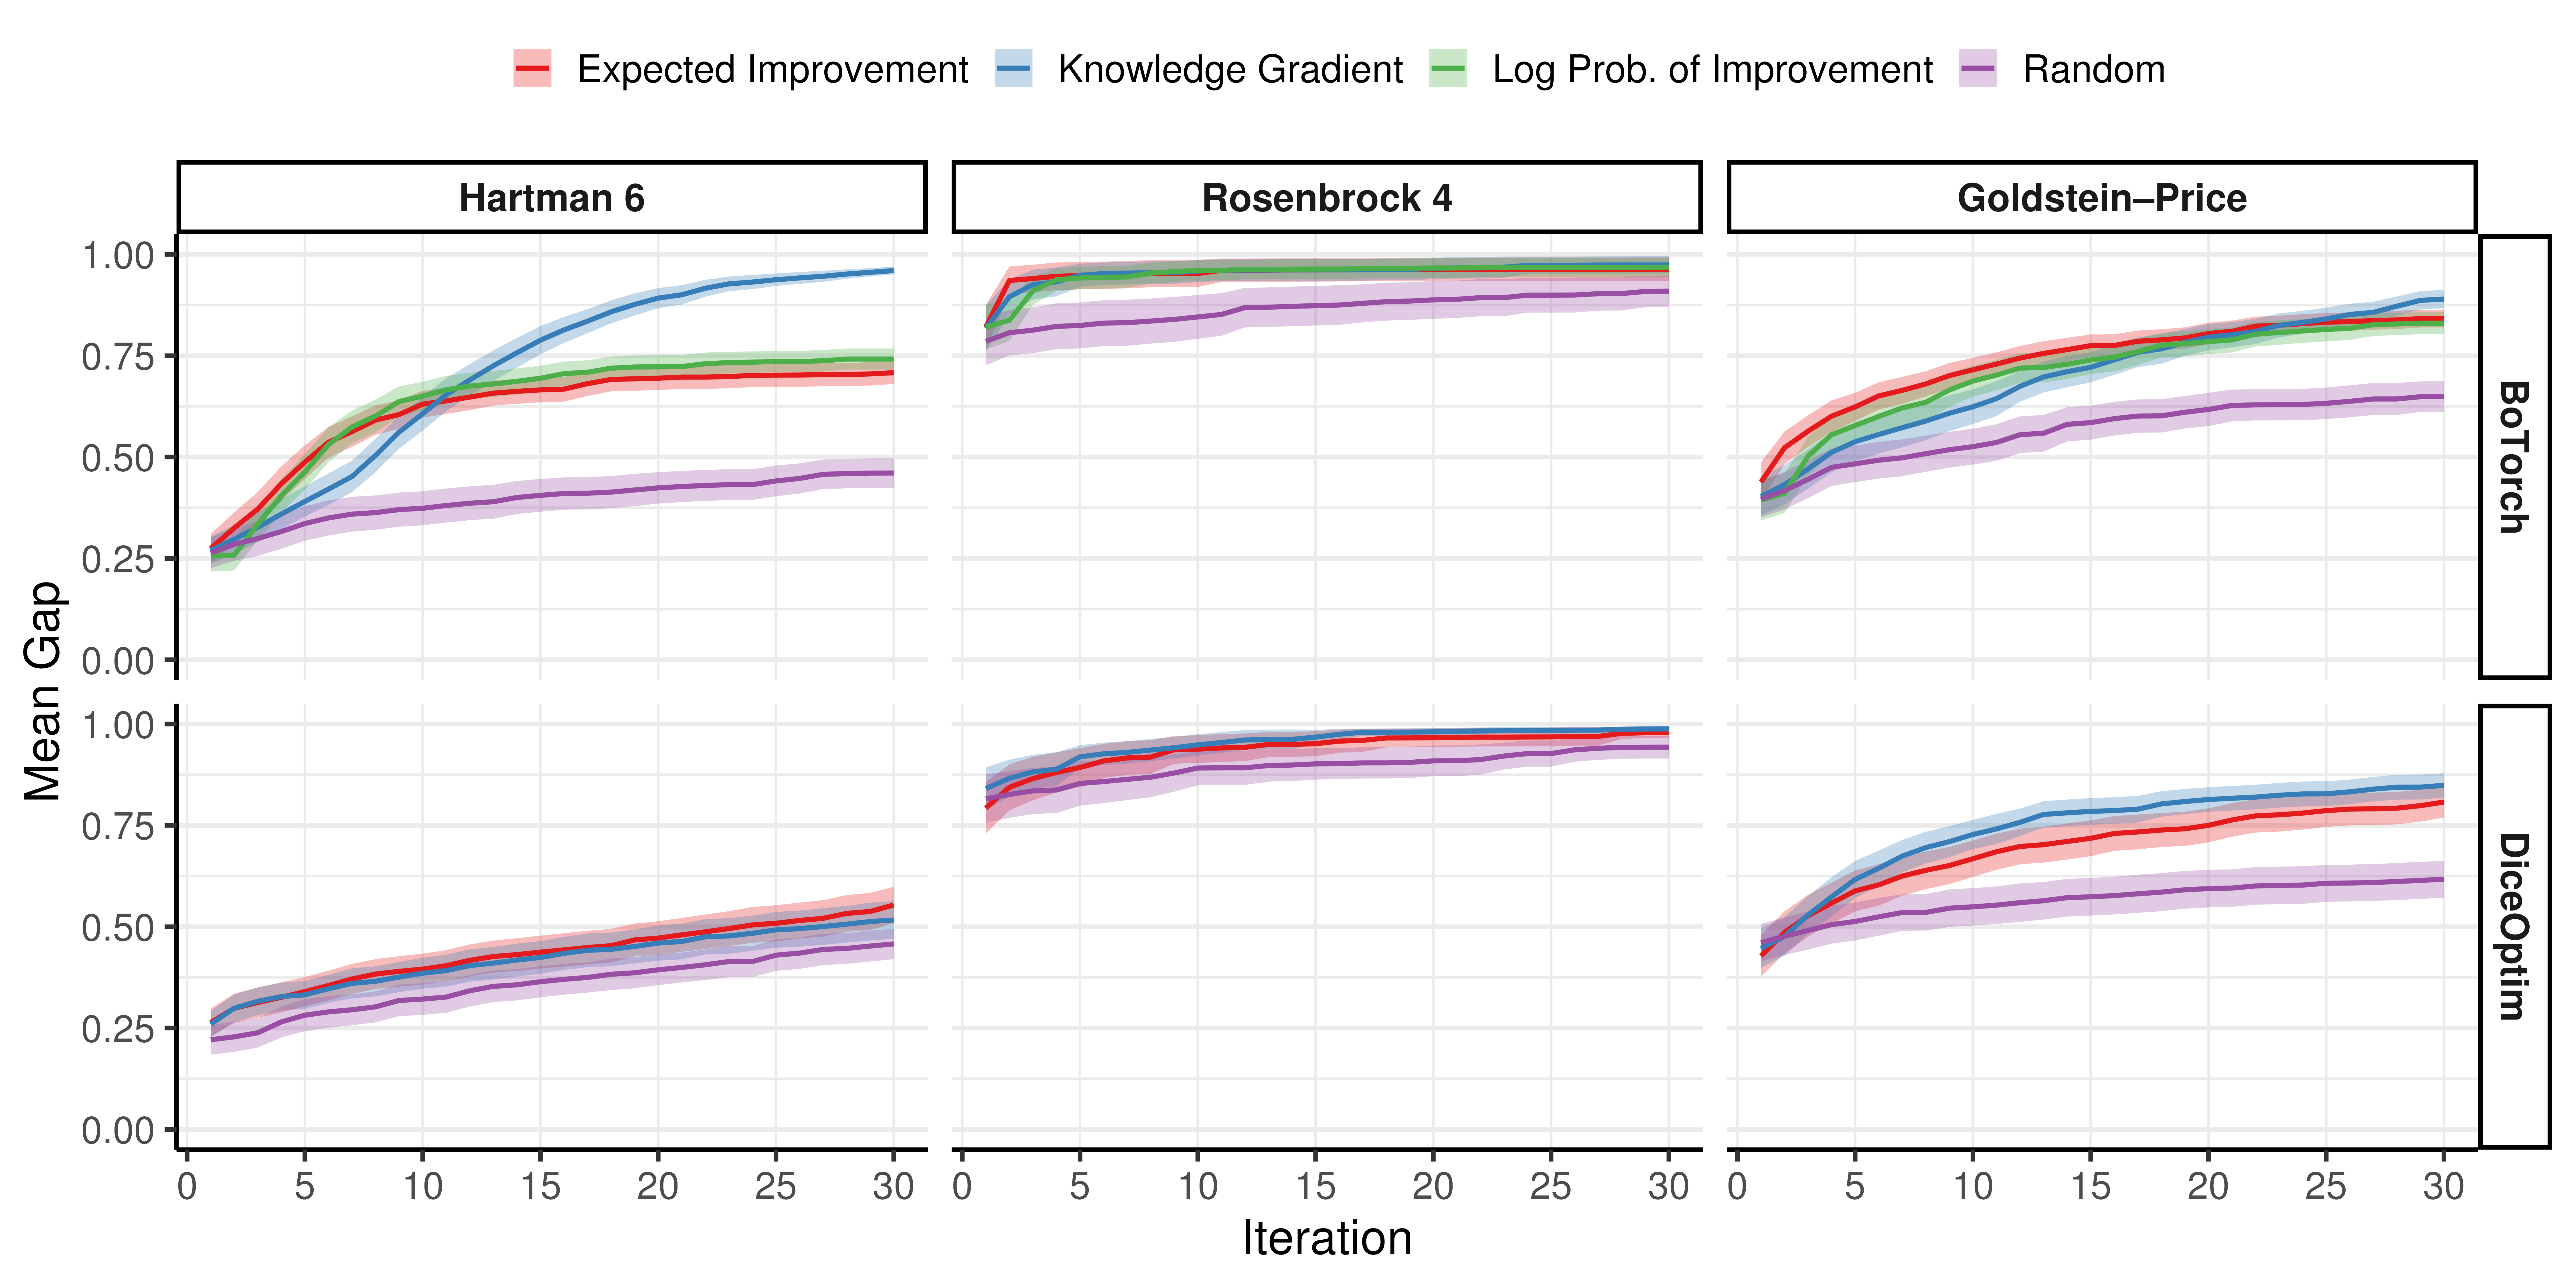
\includegraphics[width=0.99\linewidth]{output/gap_results.png}
\caption{\small \textbf{Optimization performance depends on test and acquisition functions as well as on implementation choice}. Each curve represents the overage Gap over 100 simulation runs. Shaded areas show pointwise 95\% confidence intervals. Purple curves (``Random'') refer to choosing evaluation points randomly instead of based on the maximum of some acquisition function.}
\label{fig:gap}
\end{figure}

Running time was evaluated through the average time per iteration, computed within each simulation run as the total time taken by the full BayesOpt algorithm divided by the number of iterations (30). The results are shown in Figure (\ref{fig:runtime}). The choice of acquisition function was the primary driver of the variation in running times. In particular, Knowledge Gradient was the most time-consuming case while random input choice was the fastest. Expected Improvement and (log) Probability of improvement showed intermediate running times. The BoTorch implementation was faster than DiceOptim when using Expected Improvement and slower when using either Knowledge Gradient or random input choice. While DiceOptim was particularly fast when optimizing the Rosenbrock 4 function with Knowledge Gradient, no major effects of the test function on running times were observed.

\begin{figure}[H]
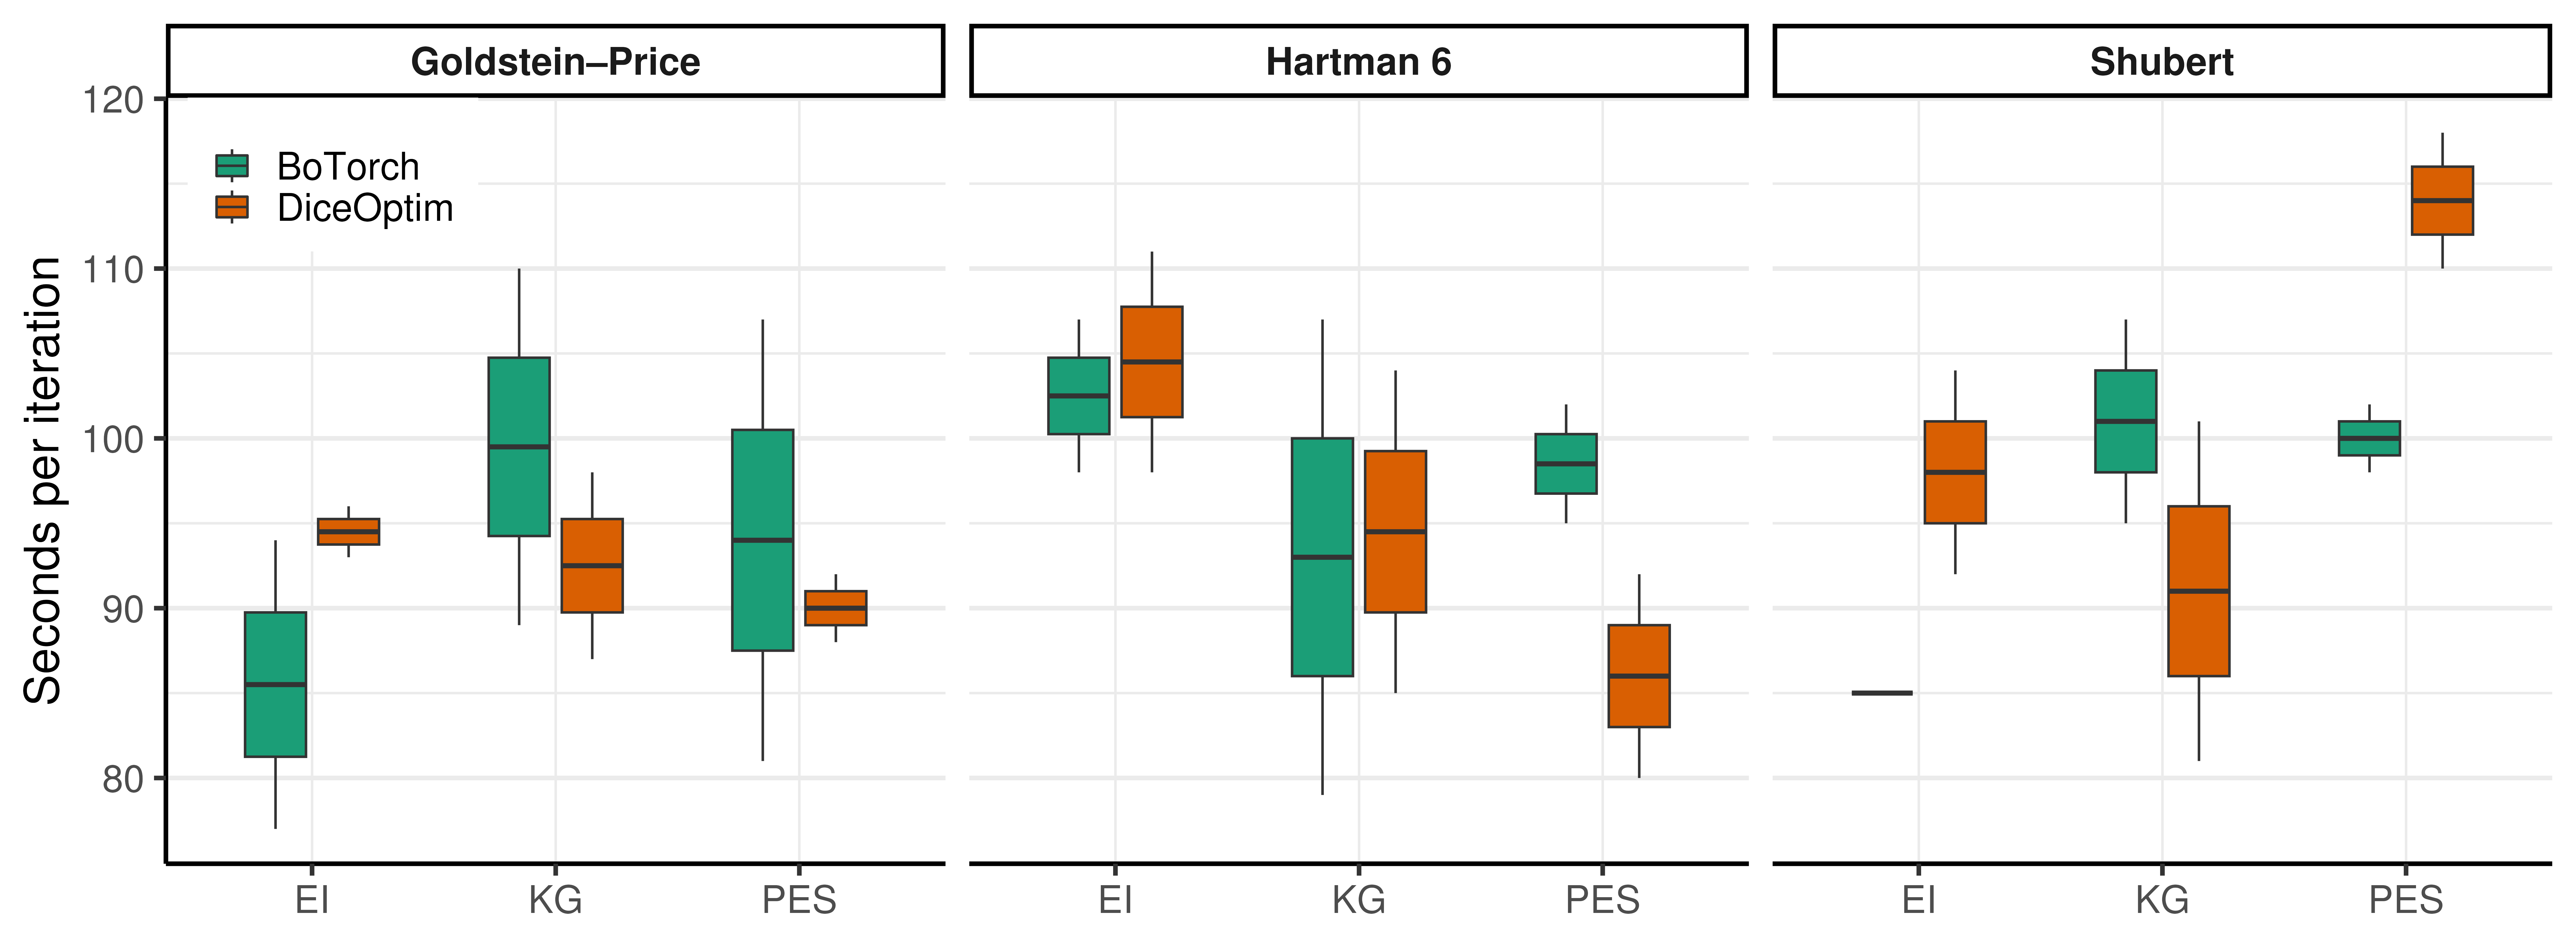
\includegraphics[width=0.99\linewidth]{output/runtime_results.png}
\caption{\small \textbf{Choice of acquisition function was the driver of variation in BayesOpt running times}. Average running time per iteration was defined as the number of seconds to run a full Bayesian Optimization procedure, divided by the total number of iterations (30). Each box summarizes the distribution of 100 observations of average running time per iteration, obtained independently from each of the 100 simulation runs. EI: Expected Improvement; KG: Knowledge Gradient; LPI: log Probability of Improvement; Random: baseline case.}
\label{fig:runtime}
\end{figure}

\subsection{Discussion}

Deploying Bayesian Optimization into practice involves a variety of decisions, from software implementation to acquisition function. Here, we report a simple simulation study to evaluate the optimization performance and efficiency of two major implementations across different acquisition functions and test objective functions. We also included a negative control ``acquisition function'' as a baseline: choosing the next evaluation point uniformly at random.

At a minimum, the benefit of BayesOpt lies in reaching global optima faster than random input choice, in terms of the number of objective function evaluations (iterations). This was the case throughout for the BoTorch implementation, but not for DiceOptim. By default, BoTorch uses GPytorch, an efficient and generic Gaussian Process library in Python \cite{Gardner2018}. Conversely, the DiceOptim employs kriging methods implemented in the \href{https://rdrr.io/cran/DiceKriging/man/km.html}{km} function from the DiceKriging R package, which requires the specification of a mean trend formula \cite{Roustant2012}. While the default formula defines a constant trend of the Kriging model, different trend structures may be optimal for different objective functions. When initially exploring both implementations, even simple linear trend formulas led to numerical issues with DiceOptim, in particular for the Hartman 6 function, unless the number of initial function evaluations $n_0$ was substantial (e.g., larger than 20). With default implementations, our results largely favoured the BoTorch implementation. Still, future work may evaluate DiceOptim performance with different mean trends, although this may require the penalized estimation method currently implemented in ``beta version'' within DiceKriging.

An interesting observation was the dependency between the best-performing acquisition function and the number of function evaluations when optimizing the Hartman 6 function with BoTorch. During initial iterations, Expected Improvement and (log) Probability of Improvement outperformed Knowledge Gradient in terms of mean Gap values. However, Knowledge Gradient became increasingly superior after 15 iterations. This suggests that the optimal acquisition function may depend not only on the objective function itself but also on the available budget of function evaluations. Knowledge Gradient may require a greater number of objective function evaluations to properly estimate posterior means and thereby improve optimization performance compared to Expected Improvement and (log) Probability of Improvement.

Finally, running times per function evaluation were comparable across test functions. The choice of acquisition function was the main driver of variation in time per iteration. Knowledge Gradient was the most time-consuming choice, likely due to being harder to optimize. While both DiceOptim and BoTorch approximate Knowledge Gradient, the version from DiceOptim was significantly faster. This might be due to different approximation approaches, different underlying acquisition function optimization routines (on top of L-BFGS-B), or different gradient computation methods (BoTorch uses automatic differentiation, while DiceOptim employs analytical gradients).

Overall, the results presented here support BoTorch as the implementation of choice for Bayesian Optimization. Importantly, the default implementation in DiceOptim may perform no better than randomly choosing points from the input space at each BayesOpt iteration. Using DiceOptim for Bayesian Optimization may require careful choice of mean trend formula and associated estimation method, beyond the implemented defaults. Provided sufficient evaluations of the objective function, Knowledge Gradient was the best-performing acquisition function. Yet, when the budget for function evaluations is very limited or when running time is critical, Expected Improvement may be preferred.